\chapter{Risultati Sperimentali}
\label{chap:Risultati sperimentali}

\section{Addestramento}
\label{sec:Addestramento}

Il modello è stato addestrato utilizzando la tecnica della \textit{cross-validation} (vedi Figura
\ref{fig:cross_validation}), con una suddivisione dei dati in cinque parti uguali (cinque folds). In
questo contesto di apprendimento supervisionato, al modello sono state fornite immagini originali
insieme alle loro corrispondenti segmentazioni effettuate manualmente.

\begin{figure}[!ht]
	\centering
	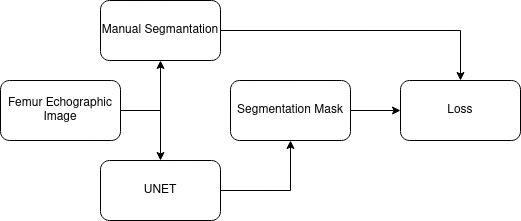
\includegraphics[width=0.7\columnwidth]{Immagini/training.png}
	\caption{Processo di addestramento del modello}
	\label{fig:addestramento_del_modello}
\end{figure}

L'addestramento è stato eseguito per 5 iterazioni (\autoref{fig:loss e accuratezza della prima porzione di dati},
\autoref{fig:loss e accuratezza della seconda porzione di dati}, \autoref{fig:loss e accuratezza della terza porzione di dati},
\autoref{fig:loss e accuratezza della quarta porzione di dati} e \autoref{fig:loss e accuratezza della quinta porzione di dati}
), utilizzando un fold diverso in ciascuna
iterazione. L'errore finale è stato calcolato come la media degli errori ottenuti in ciascuna delle
cinque iterazioni.

L'errore finale è stato calcolato mettendo a confronto la segmentazione ottenuta dal modello con la
segmentazione manuale (\autoref{fig:addestramento_del_modello}).


\begin{figure}[!ht]
	\centering
	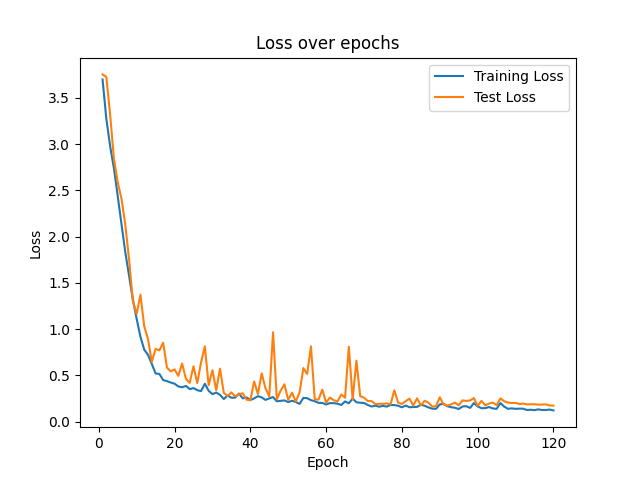
\includegraphics[width=0.4\columnwidth]{Immagini/fold_0_loss.png} 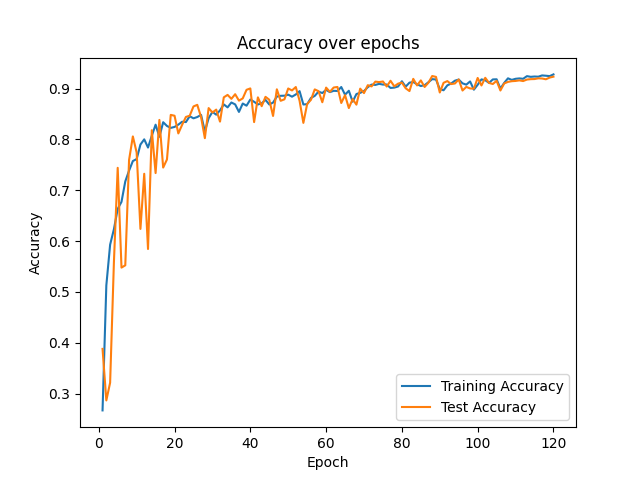
\includegraphics[width=0.4\columnwidth]{Immagini/fold_0_accuracy.png}
	\caption{Errore e accuratezza della prima porzione di dati}
	\label{fig:loss e accuratezza della prima porzione di dati}
\end{figure}

\begin{figure}
	\centering
	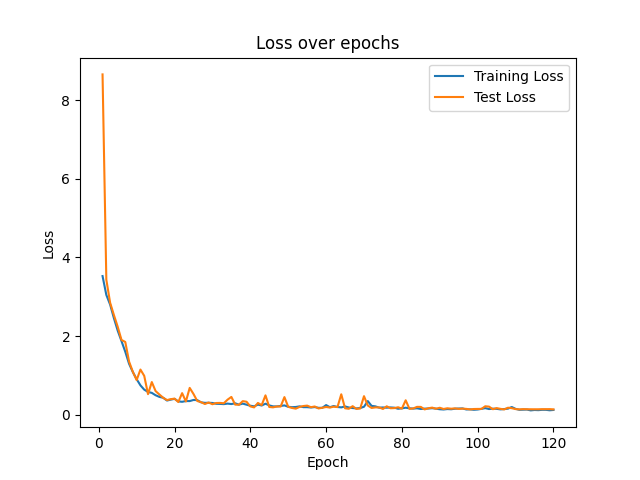
\includegraphics[width=0.4\columnwidth]{Immagini/fold_1_loss.png} 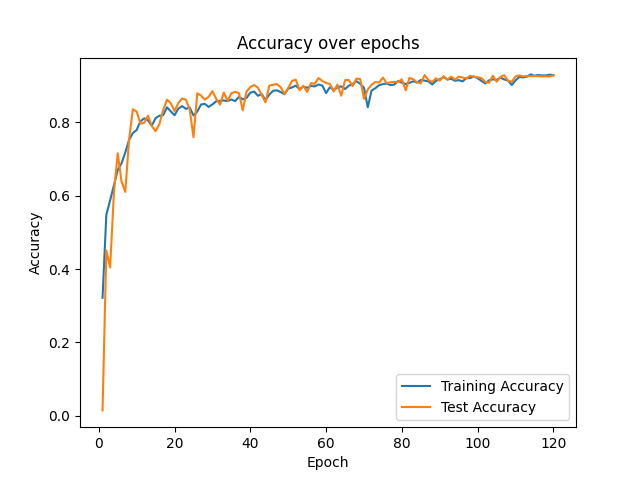
\includegraphics[width=0.4\columnwidth]{Immagini/fold_1_accuracy.png}
	\caption{Errore e accuratezza della seconda porzione di dati}
	\label{fig:loss e accuratezza della seconda porzione di dati}
\end{figure}

\begin{figure}
	\centering
	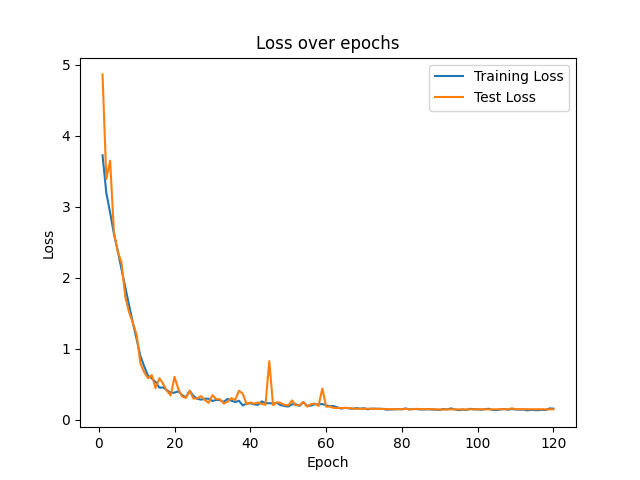
\includegraphics[width=0.4\columnwidth]{Immagini/fold_2_loss.png} 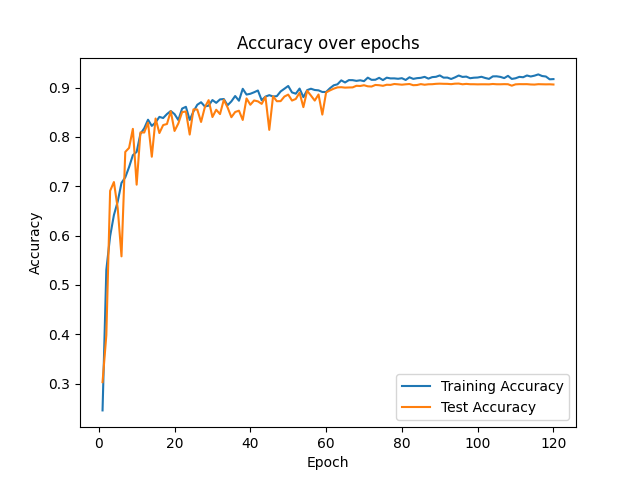
\includegraphics[width=0.4\columnwidth]{Immagini/fold_2_accuracy.png}
	\caption{Errore e accuratezza della terza porzione di dati}
	\label{fig:loss e accuratezza della terza porzione di dati}
\end{figure}

\begin{figure}
	\centering
	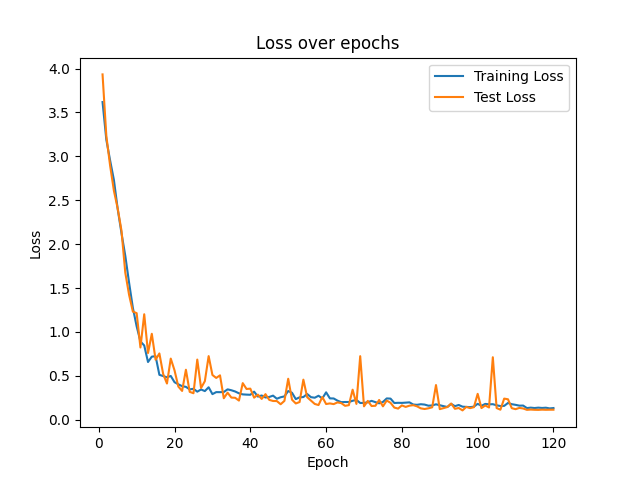
\includegraphics[width=0.4\columnwidth]{Immagini/fold_3_loss.png} 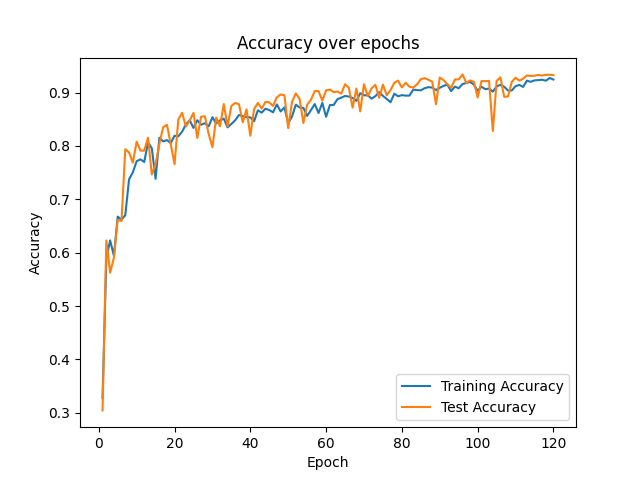
\includegraphics[width=0.4\columnwidth]{Immagini/fold_3_accuracy.png}
	\caption{Errore e accuratezza della quarta porzione di dati}
	\label{fig:loss e accuratezza della quarta porzione di dati}
\end{figure}

\begin{figure}
	\centering
	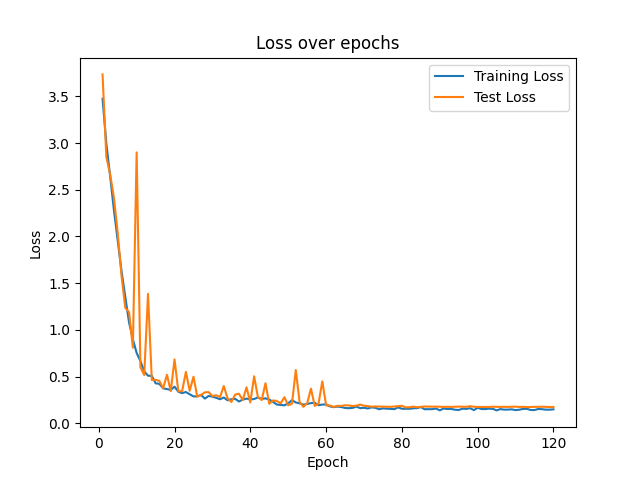
\includegraphics[width=0.4\columnwidth]{Immagini/fold_4_loss.png} 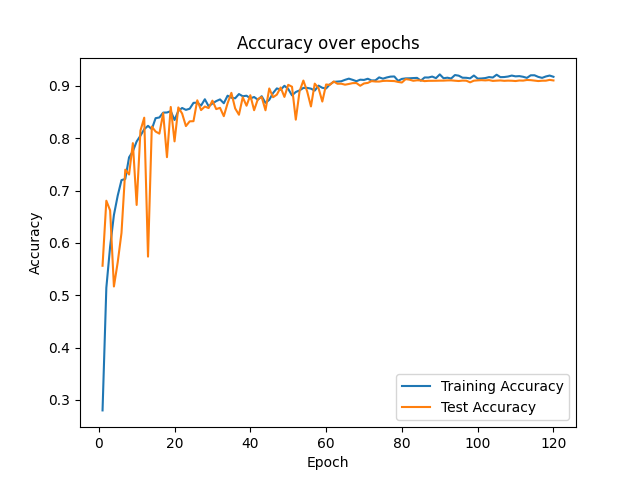
\includegraphics[width=0.4\columnwidth]{Immagini/fold_4_accuracy.png}
	\caption{Errore e accuratezza della quinta porzione di dati}
	\label{fig:loss e accuratezza della quinta porzione di dati}
\end{figure}


L'\textbf{errore} complessivo è stato calcolato come media degli errori ottenuti in ciascuna delle
cinque iterazioni di addestramento, utilizzando la formula \ref{eq:dice_bce_loss_complete}. Il
risultato è un errore medio del \textbf{$7.9\%$}.

Parallelamente, l'\textbf{accuratezza} complessiva è stata calcolata come la media delle accuratezze
ottenute in ciascuna iterazione, impiegando la formula \ref{eq:iou}. Ciò ha portato a un'accuratezza
media del \textbf{$92.1\%$}.

Oltre alle analisi quantitative, è stato fondamentale condurre analisi qualitative sulla
segmentazione ottenuta dal modello, specialmente considerando il suo impiego in ambito medico per la
segmentazione dei femori.

Nelle immagini seguenti viene riportato uno delle immagini prese in considerazione per
l'addestramento del modello e vengono mostrate le segmentazione manuali, le segmentazioni ottenute
dal modello e la differenze nella classificazione dei pixel tra le due segmentazioni.


\begin{figure}[!ht]
	\centering
	\begin{minipage}{0.32\textwidth}
		\centering
		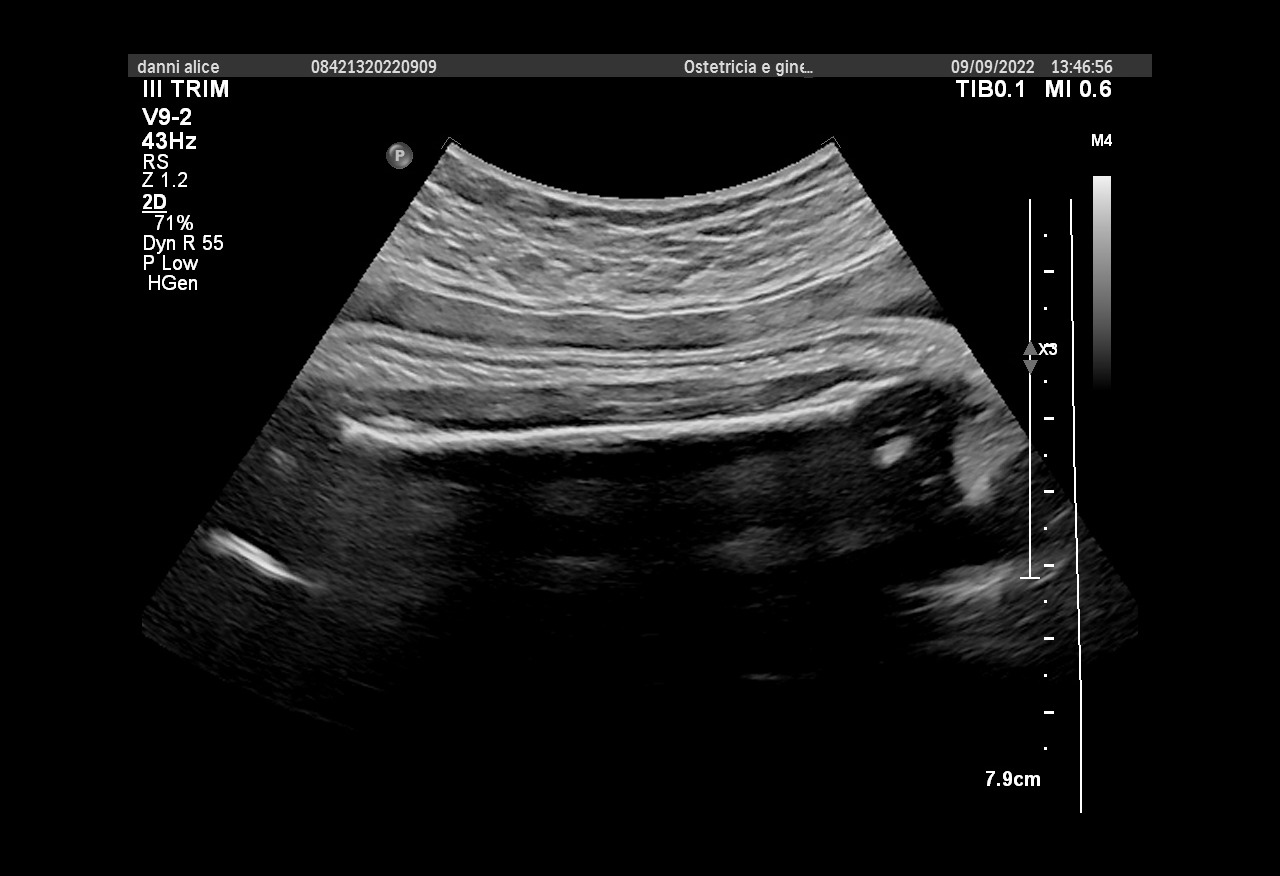
\includegraphics[width=\linewidth]{Immagini/image.png}
	\end{minipage}
	\hfill % ensures equal spacing
	\begin{minipage}{0.32\textwidth}
		\centering
		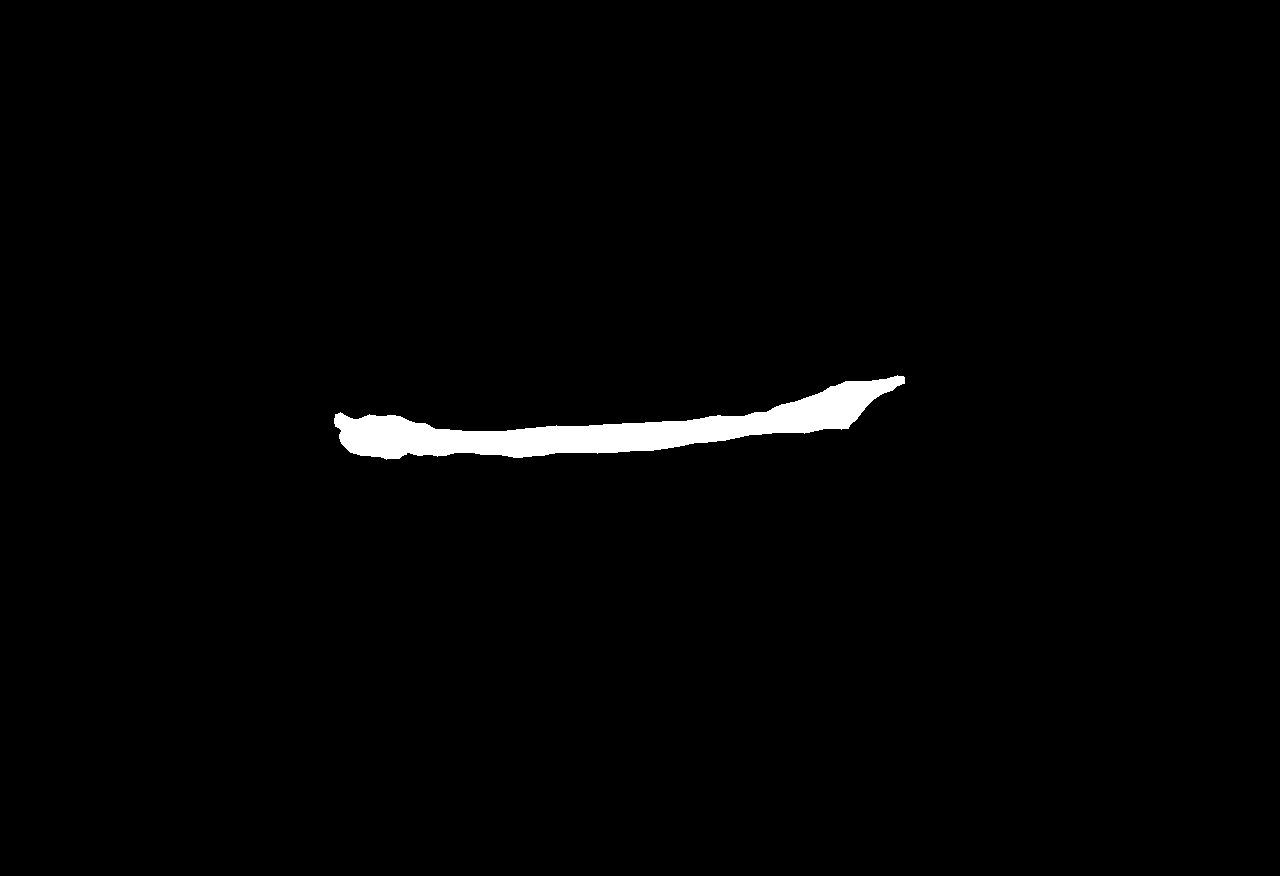
\includegraphics[width=\linewidth]{Immagini/mask.png}
	\end{minipage}
	\hfill % ensures equal spacing
	\begin{minipage}{0.32\textwidth}
		\centering
		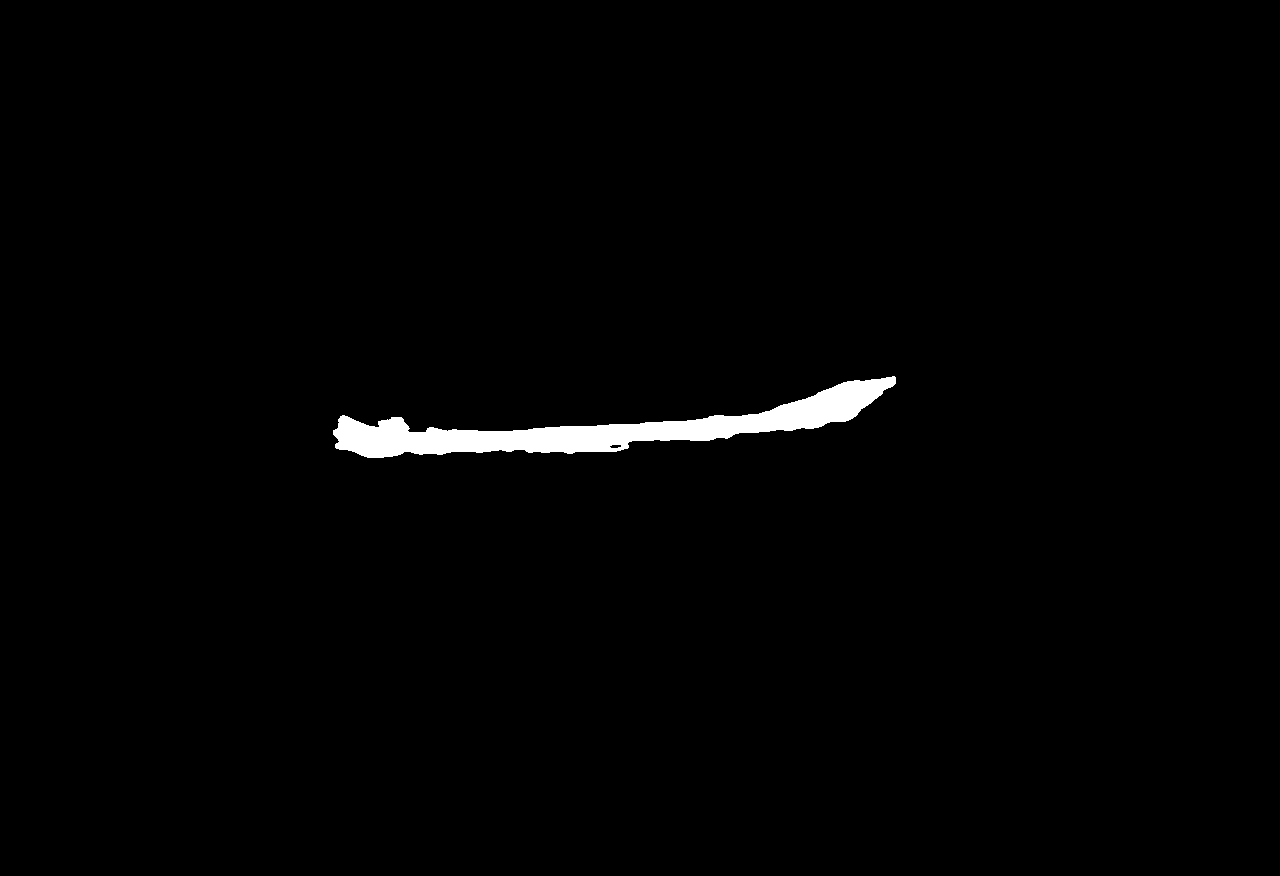
\includegraphics[width=\linewidth]{Immagini/prediction.png}
	\end{minipage}

	\caption{Immagine originale, segmentazione manuale e segmentazione del modello}
	\label{fig:risultati_quantitativi}
\end{figure}




Per confermare l'efficacia del modello nella segmentazione delle immagini, si è proceduto con
l'analisi della distribuzione dei pixel. Questa analisi confronta direttamente la segmentazione
manuale con quella ottenuta dal modello. L'obiettivo è dimostrare che la distribuzione dei pixel
nelle segmentazioni del modello corrisponde strettamente a quella delle segmentazioni manuali,
indicando così una segmentazione accurata.


\begin{figure}[!ht]
	\centering
	\begin{minipage}{0.32\textwidth}
		\centering
		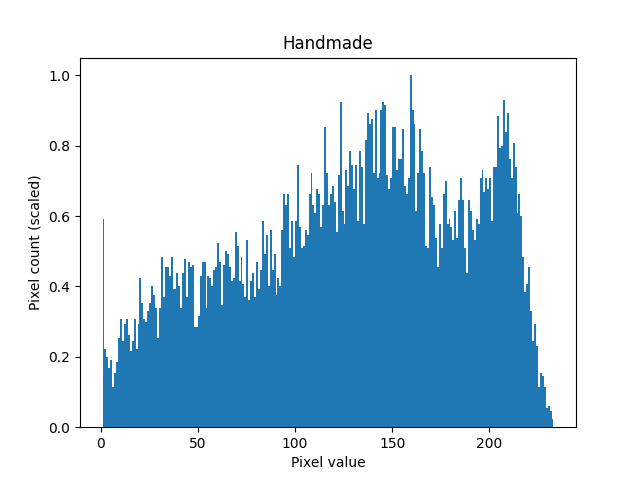
\includegraphics[width=\linewidth]{Immagini/handmade_scaled_hist.png}
	\end{minipage}
	\hfill % ensures equal spacing
	\begin{minipage}{0.32\textwidth}
		\centering
		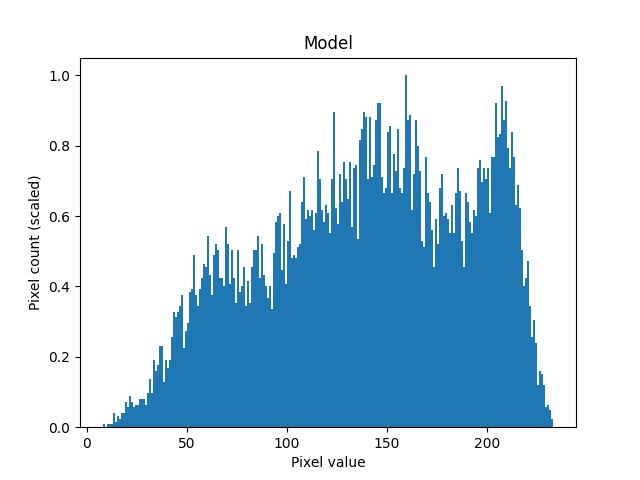
\includegraphics[width=\linewidth]{Immagini/model_scaled_hist.png}
	\end{minipage}
	\hfill % ensures equal spacing
	\begin{minipage}{0.32\textwidth}
		\centering
		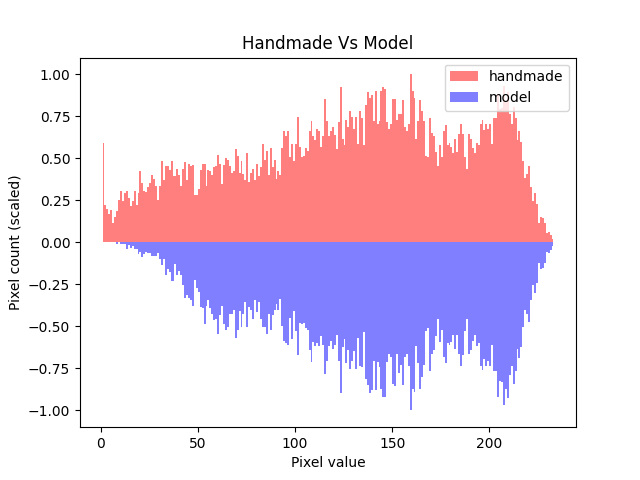
\includegraphics[width=\columnwidth]{Immagini/handmade_vs_model_scaled.png}
	\end{minipage}
	\caption{Distribuzione Intensità dei pixel della segmentazione manuale, della segmentazione del modello e confronto tra le due}
	\label{fig:grafico_distribution_value}
\end{figure}


I risultati ( \autoref{fig:risultati_quantitativi} e \autoref{fig:grafico_distribution_value} ) mostrano che la distribuzione dei pixel nelle segmentazioni generate dal modello si
allinea strettamente a quella delle segmentazioni manuali, suggerendo che il modello è in grado di
segmentare le immagini con precisione.


Dall'analisi dei risultati sia qualitativi che quantitativi, emerge che il modello mostra una
performance molto promettente. In particolare, si evidenzia che il modello supera abbondantemente
un'accuratezza del $90\%$, offrendo un ampio margine per ulteriori miglioramenti attraverso
l'incremento del numero di immagini disponibili per l'addestramento.

Degno di nota è la non necessità di effettuare ulteriori segmentazioni manuali per espandere il set
di addestramento. Le nuove immagini raccolte possono essere segmentate automaticamente utilizzando il
modello e poi impiegate per rafforzare ulteriormente il processo di addestramento. Questo approccio
non solo semplifica il processo di raccolta dati, ma accelera anche la possibilità di miglioramento
e adattamento del modello a nuovi dati.


\section{Analisi del Nuovo Ecografo}
\label{sec:analisi_nuovo_ecografo}

In questa sezione, esploriamo l'impatto dell'introduzione di un nuovo ecografo sulle prestazioni del
nostro modello di segmentazione. Questo nuovo strumento rappresenta una sfida significativa per il
modello, in quanto introduce un set di dati con caratteristiche visive diverse da quelle su cui è
stato originariamente addestrato.

\subsection{Confronto delle Immagini}
\label{subsec:confronto_immagini}

Sono state fornite al modello alcune immagini acquisite dal nuovo ecografo. Queste non hanno subito
nessun tipo di elaborazione, ma sono state direttamente segmentate dal modello.


\begin{figure}[!ht]
	\centering
	\begin{minipage}{0.32\textwidth}
		\centering
		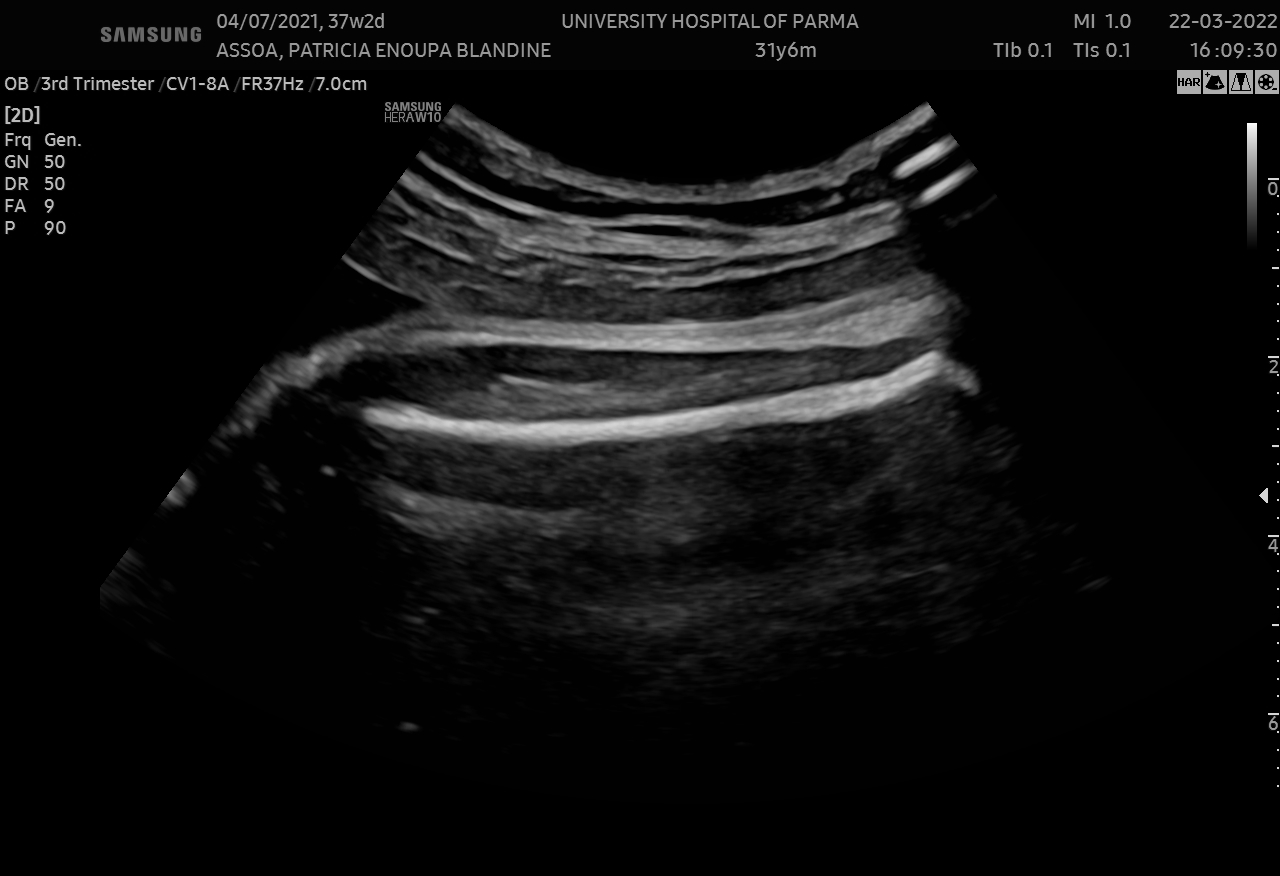
\includegraphics[width=\textwidth]{./Immagini/nuovo_ecografo_results/0_image.png}
	\end{minipage}
	\hfill % ensures equal spacing
	\begin{minipage}{0.32\textwidth}
		\centering
		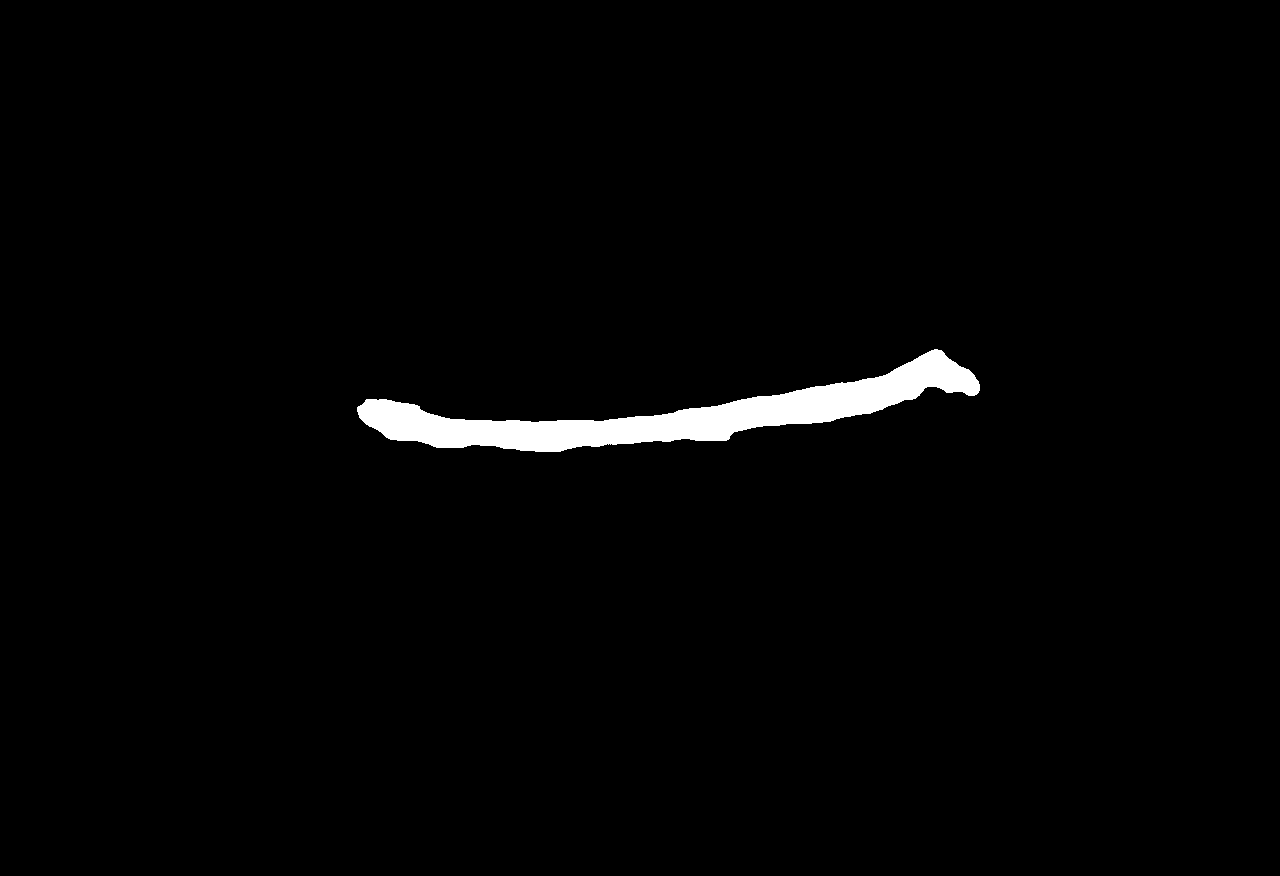
\includegraphics[width=\textwidth]{./Immagini/nuovo_ecografo_results/0_mask.png}
	\end{minipage}
	\hfill % ensures equal spacing
	\begin{minipage}{0.32\textwidth}
		\centering
		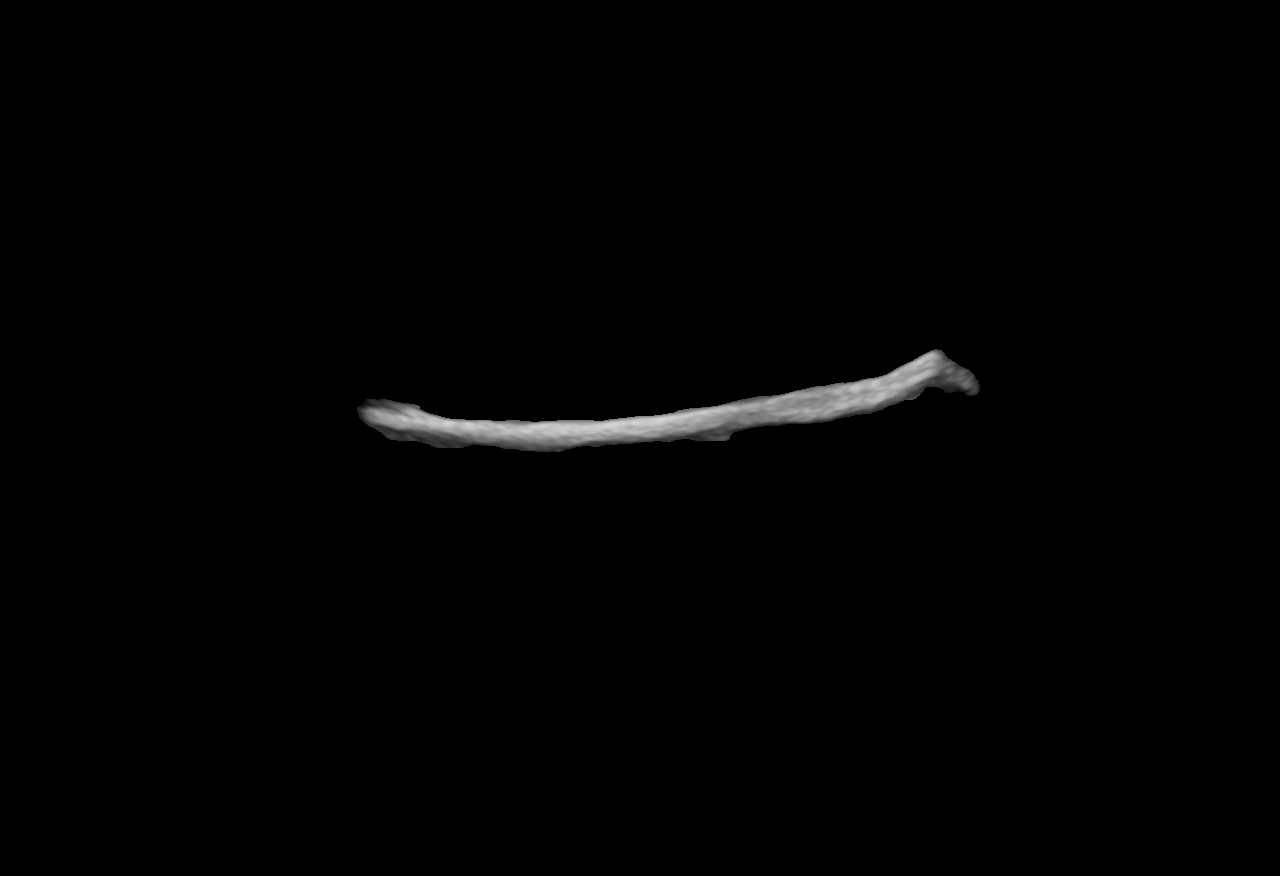
\includegraphics[width=\textwidth]{./Immagini/nuovo_ecografo_results/0_extracted_femur.png}
	\end{minipage}
\end{figure}

\begin{figure}[!ht]
	\centering
	\begin{minipage}{0.32\textwidth}
		\centering
		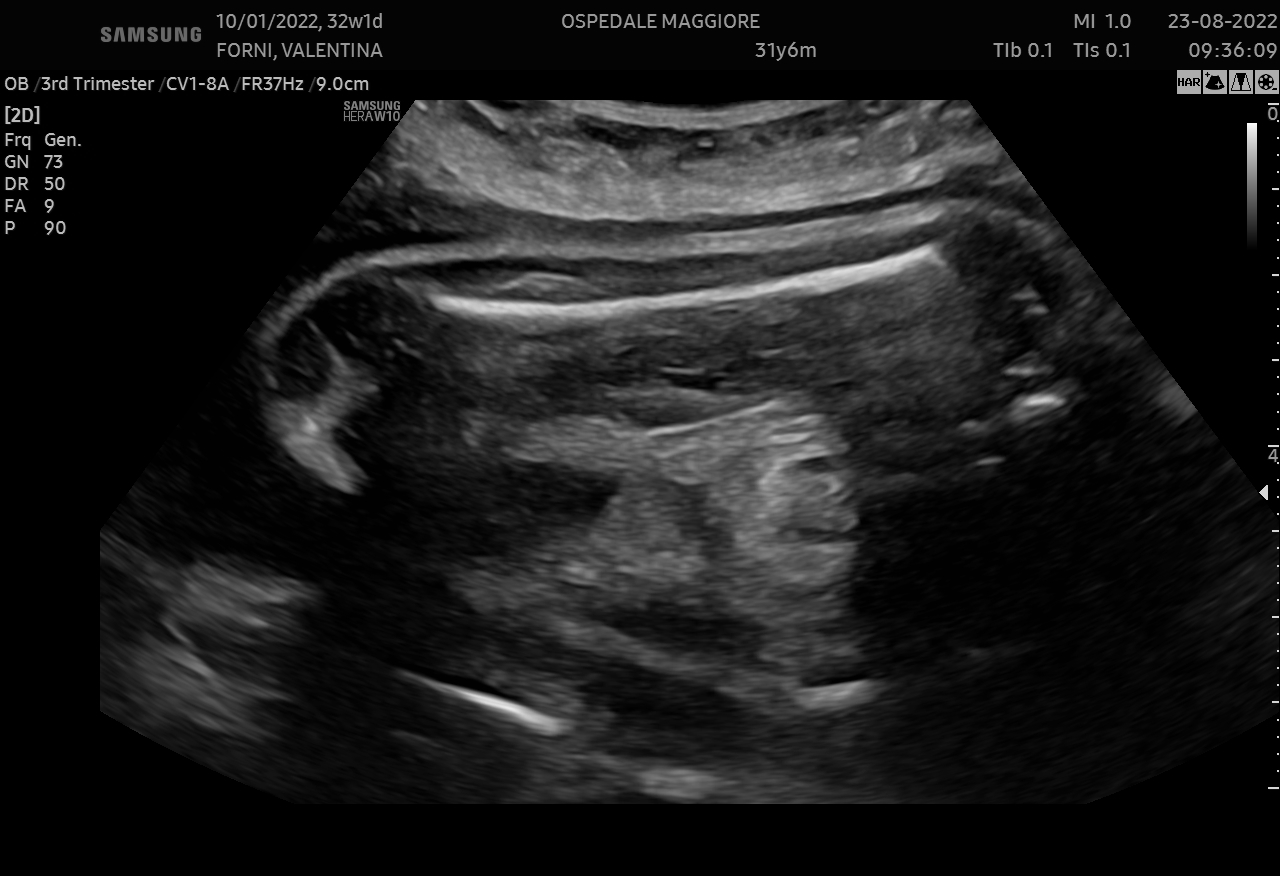
\includegraphics[width=\textwidth]{./Immagini/nuovo_ecografo_results/4_image.png}
	\end{minipage}
	\hfill % ensures equal spacing
	\begin{minipage}{0.32\textwidth}
		\centering
		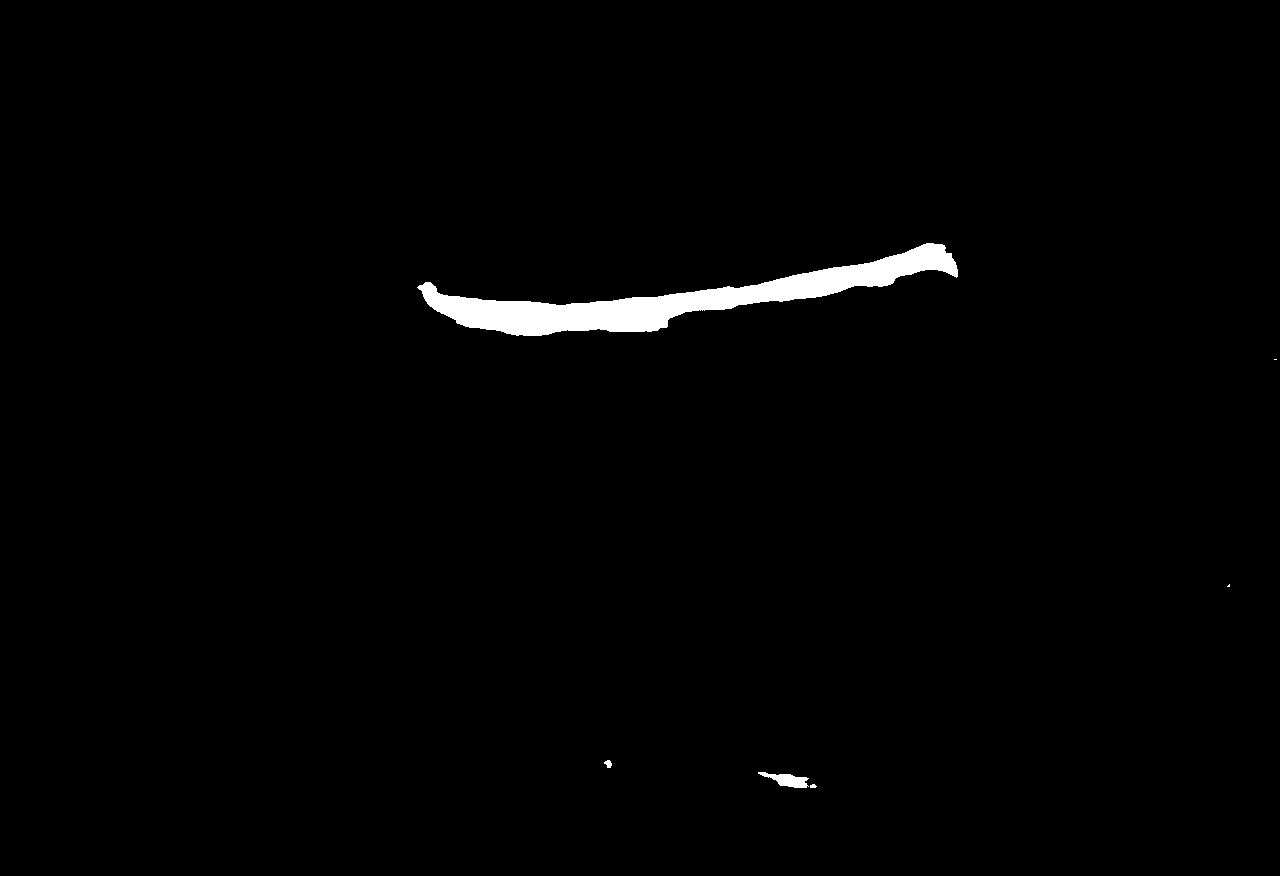
\includegraphics[width=\textwidth]{./Immagini/nuovo_ecografo_results/4_mask.png}
	\end{minipage}
	\hfill % ensures equal spacing
	\begin{minipage}{0.32\textwidth}
		\centering
		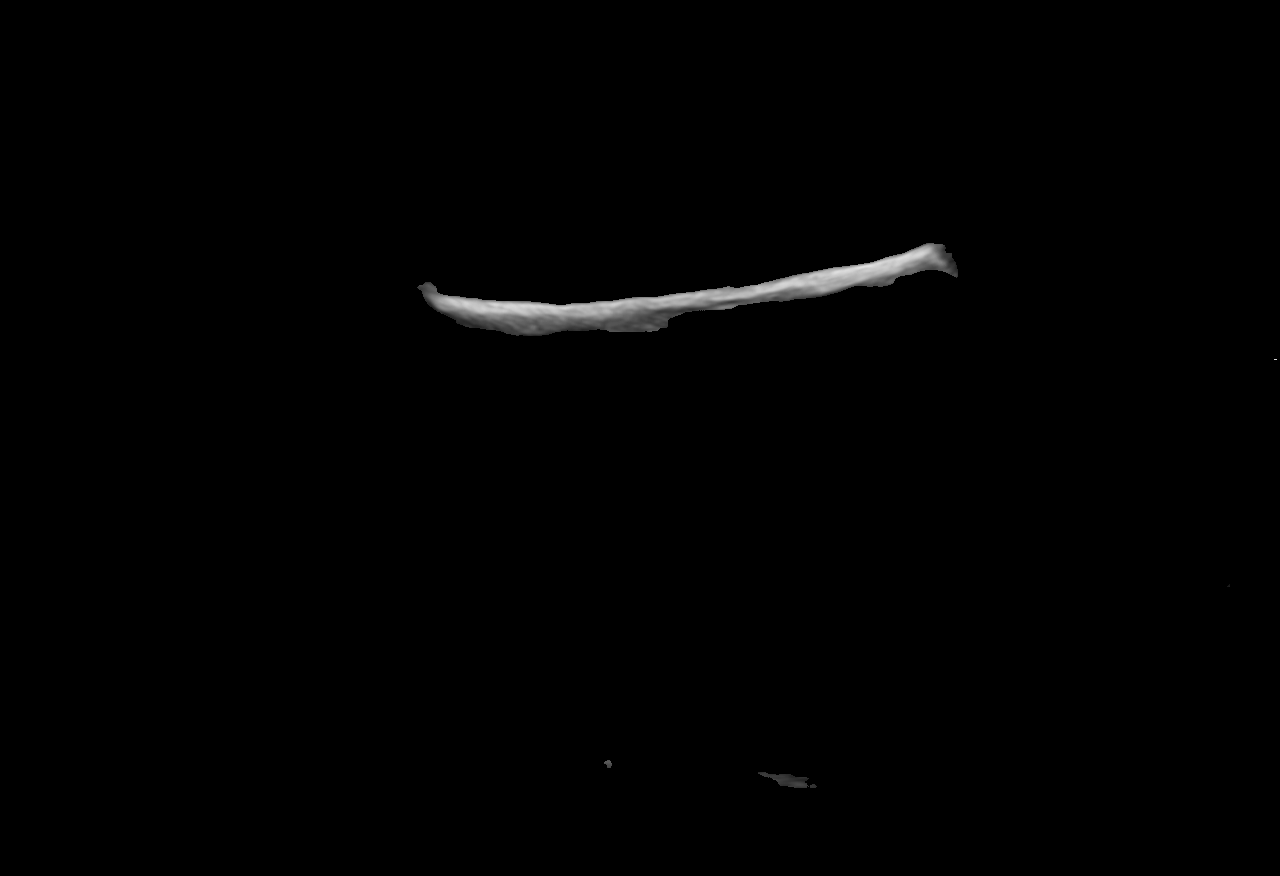
\includegraphics[width=\textwidth]{./Immagini/nuovo_ecografo_results/4_extracted_femur.png}
	\end{minipage}
\end{figure}

\begin{figure}[!ht]
	\centering
	\begin{minipage}{0.32\textwidth}
		\centering
		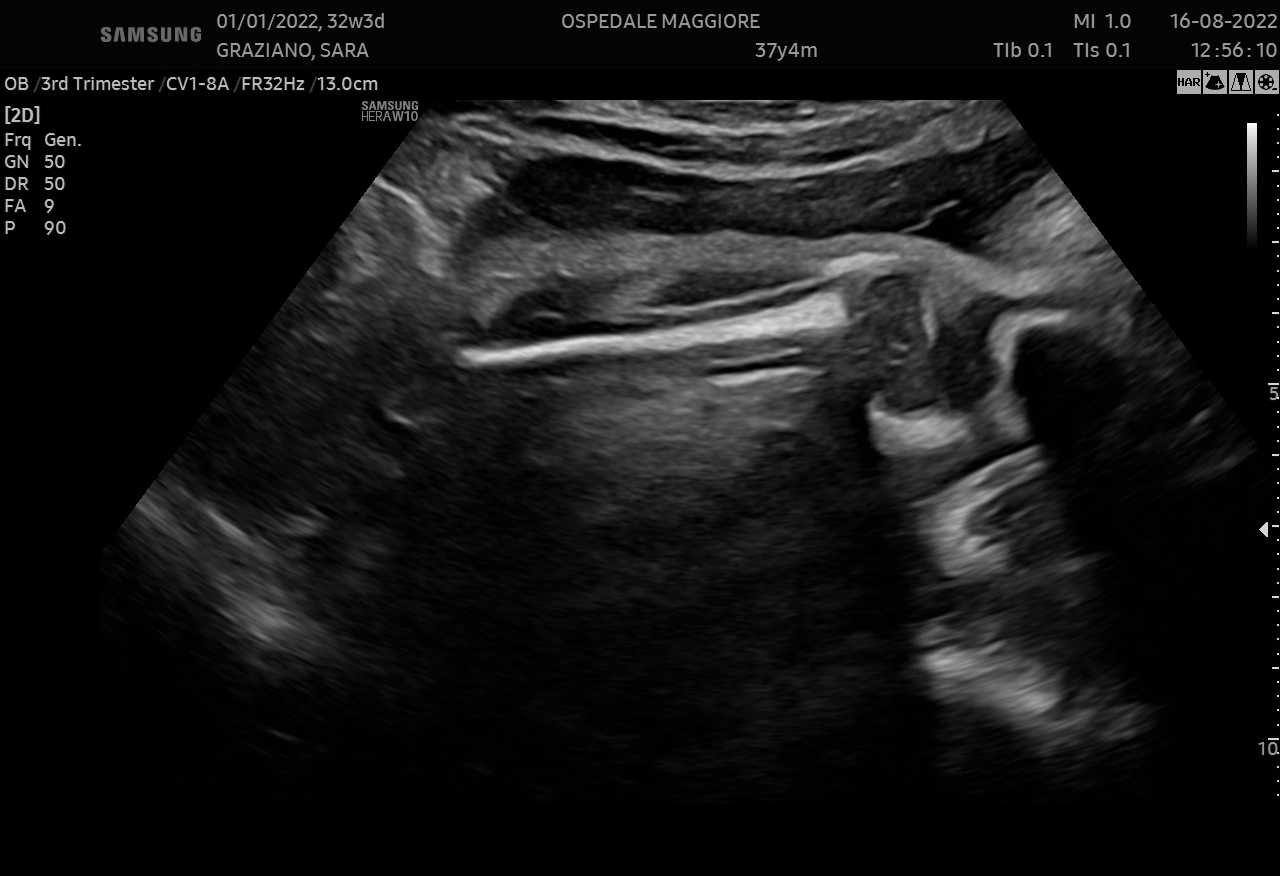
\includegraphics[width=\textwidth]{./Immagini/nuovo_ecografo_results/3_image.png}
	\end{minipage}
	\hfill % ensures equal spacing
	\begin{minipage}{0.32\textwidth}
		\centering
		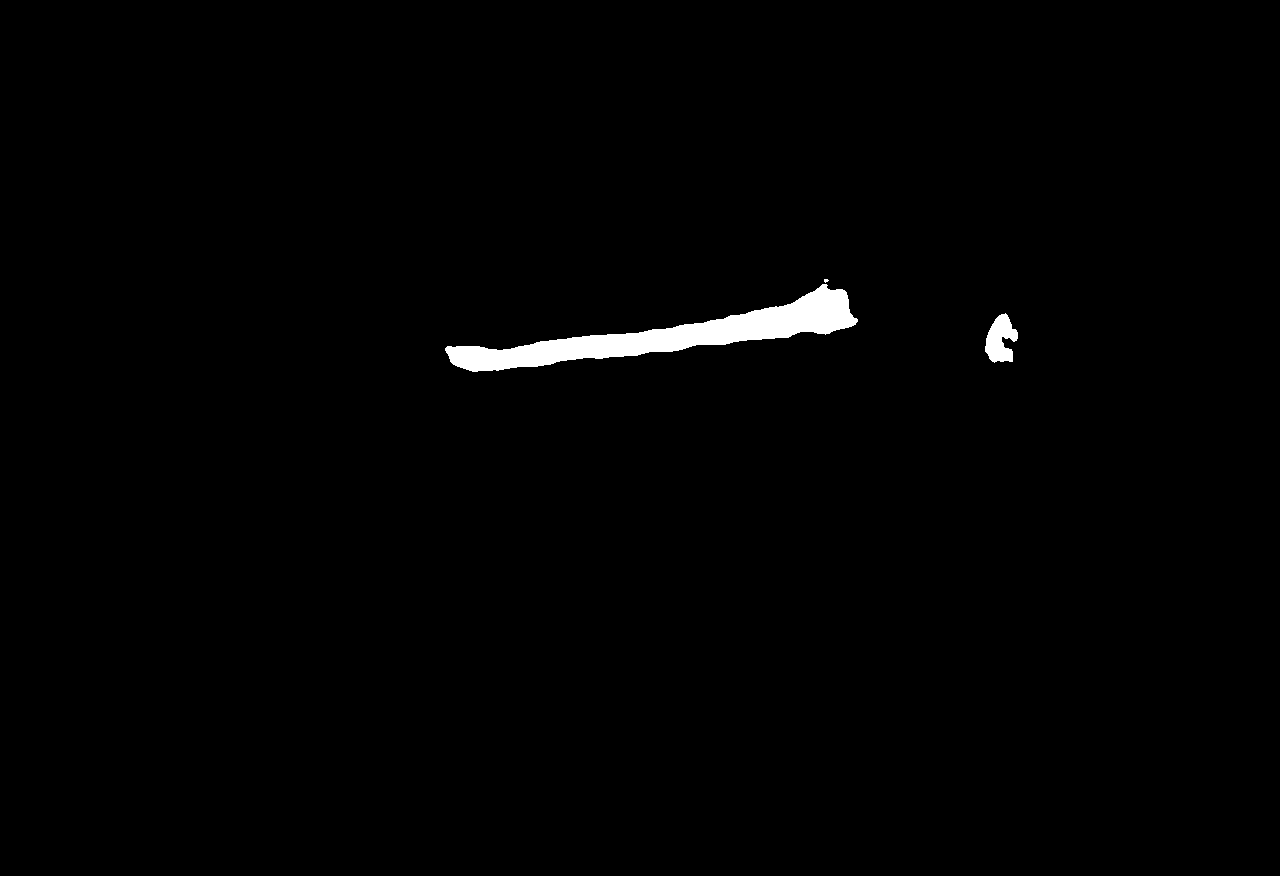
\includegraphics[width=\textwidth]{./Immagini/nuovo_ecografo_results/3_mask.png}
	\end{minipage}
	\hfill % ensures equal spacing
	\begin{minipage}{0.32\textwidth}
		\centering
		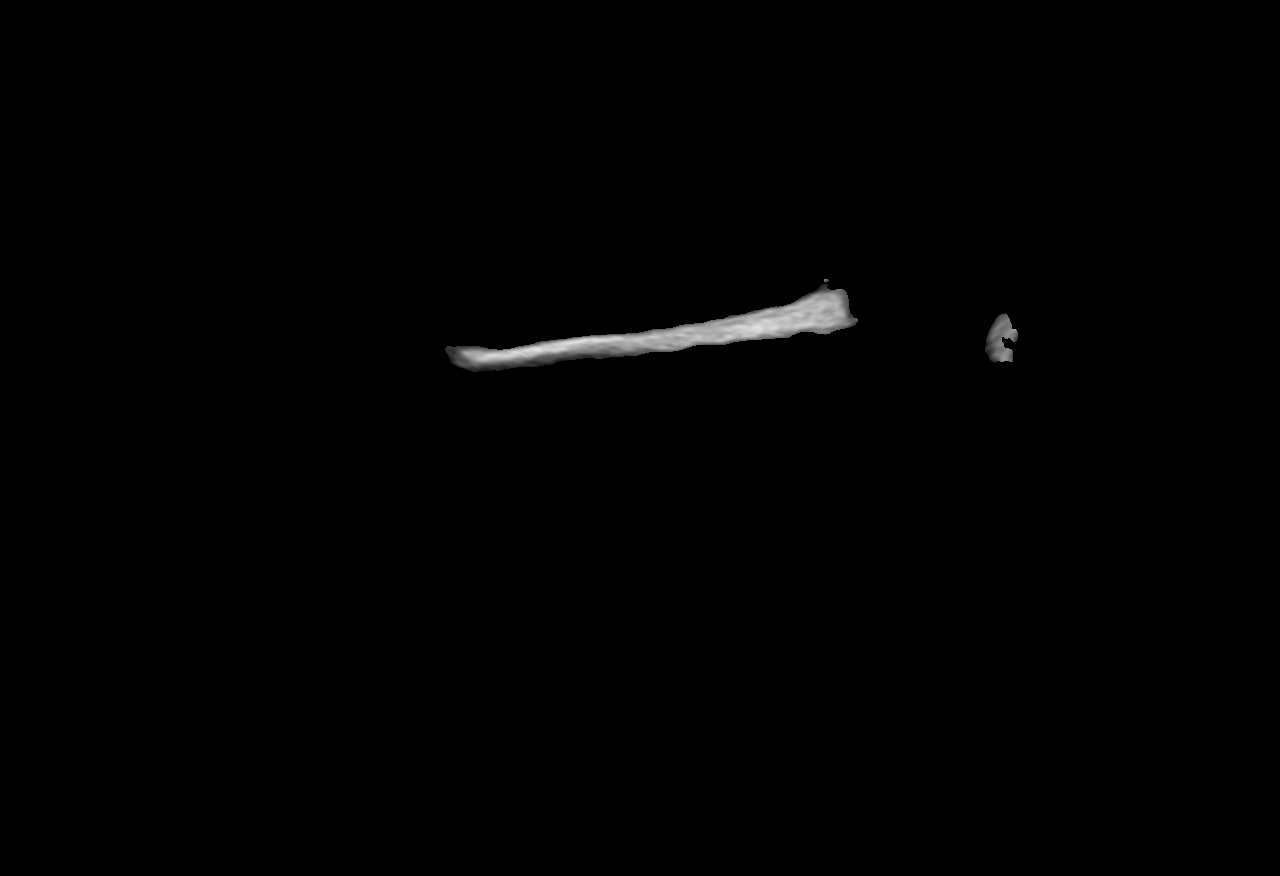
\includegraphics[width=\textwidth]{./Immagini/nuovo_ecografo_results/3_extracted_femur.png}
	\end{minipage}
	\caption{Immagine Originale, Maschera di segmentazione ottenuta dal modello e Risultato finale a seguito dell'estrazione del femore}
	\label{fig:risultati_nuovo_ecografo}
\end{figure}

\subsection{Analisi della Distribuzione dei Valori}
\label{subsec:analisi_distribuzione_valori}
% Abbiamo inoltre esaminato la distribuzione dei valori nelle immagini acquisite dal nuovo ecografo
% per comprendere meglio come il modello gestisce le nuove informazioni.

\begin{figure}[!ht]
	\centering
	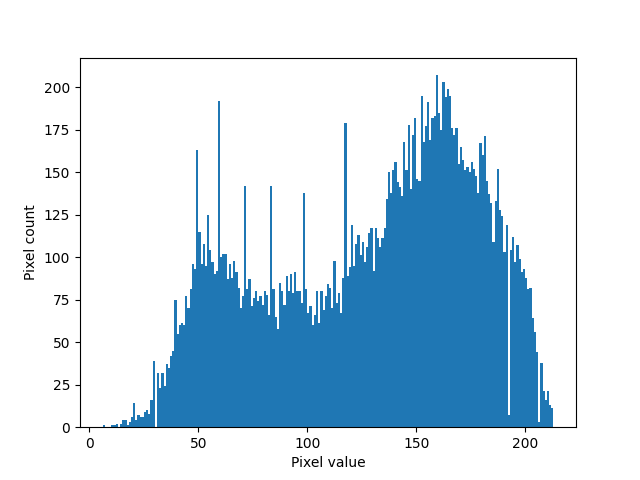
\includegraphics[width=0.45\textwidth]{./Immagini/nuovo_ecografo_results/hist_0_distribution_value.csv.png}
	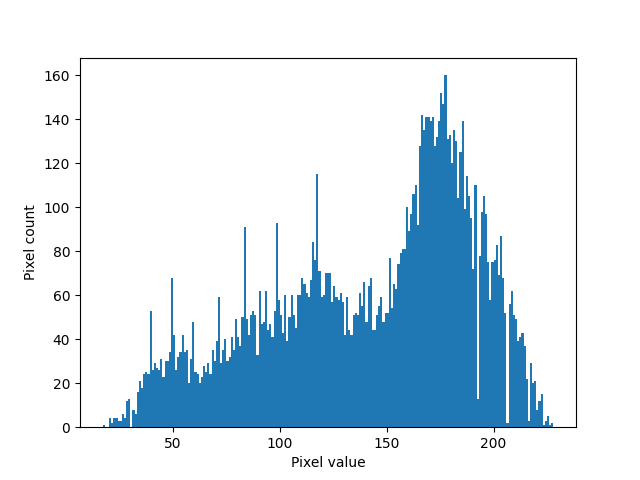
\includegraphics[width=0.45\textwidth]{./Immagini/nuovo_ecografo_results/hist_3_distribution_value.csv.png}
	\caption{Distribuzione dei Valori}
	\label{fig:distribuzione_valori}
\end{figure}

Una prima analisi qualitativa ( \autoref{fig:risultati_nuovo_ecografo} ) permette di osservare che il modello è in grado di segmentare le immagini acquisite dal nuovo ecografo.

Sono state analizzate le distribuzioni dei valori delle immagini acquisite dal
nuovo ecografo ( \autoref{fig:distribuzione_valori} ). Ponendole a confronto con le distribuzioni ottenute dal'
ecografo precedentemente utilizzato (\autoref{fig:grafico_distribution_value}), è possibile osservare che le immagini acquisite dal nuovo ecografo sono analizzabili
dal modello.

Tenendo in considerazione che il modello non è stato addestrato su questo specifico set ne su
immagini di questo specifico ecografo, è possibile notare che la distribuzione dei valori è molto
simile a quella delle immagini utilizzate per l'addestramento. Questo suggerisce che il modello è
in grado di gestire con efficacia le nuove informazioni.



% \subsection{Risultati Quantitativi}
% \label{subsec:risultati_quantitativi}
% Di seguito sono riportati i risultati quantitativi derivanti dall'analisi delle immagini del nuovo
% ecografo.
%
% \begin{table}[ht]
% 	\centering
% 	\begin{tabular}{|l|c|c|}
% 		\hline
% 		\textbf{Immagine} & \textbf{Media} & \textbf{Deviazione Standard} \\
% 		\hline
% 		\hline
% 		0                 & 128.225        & 47.961                       \\ \hline
% 		1                 & 119.319        & 46.750                       \\ \hline
% 		2                 & 175.710        & 41.832                       \\ \hline
% 		3                 & 141.379        & 47.968                       \\ \hline
% 		4                 & 129.142        & 50.137                       \\ \hline
% 		5                 & 91.6911        & 38.671                       \\ \hline
% 		6                 & 110.249        & 48.143                       \\ \hline
% 		7                 & 115.113        & 43.262                       \\ \hline
% 		8                 & 155.277        & 51.628                       \\ \hline
% 		9                 & 114.937        & 53.817                       \\ \hline
% 		10                & 145.433        & 57.311                       \\ \hline
% 		11                & 152.924        & 51.922                       \\ \hline
% 		12                & 128.146        & 53.493                       \\ \hline
% 	\end{tabular}
% 	\caption{Risultati Sperimentali}
% 	\label{tab:risultati_sperimentali}
% \end{table}

% \subsection{Discussione}
% \label{subsec:discussione}
%
% I risultati dell'addestramento permettono di concludere che il modello è in grado di gestire con
% efficacia set di dati diversi da quelli utilizzati per l'addestramento. Questo suggerisce un
% potenziale significativo per miglioramenti attraverso un addestramento mirato, che potrebbe affinare
% ulteriormente la capacità del modello di gestire con efficacia set di dati simili.
%
% Sottolineando il fatto che il modello non \`e specificamente addestrato su questi dati, la sua
% performance qualitativa appare accettabile. Ciò suggerisce un potenziale significativo per
% miglioramenti attraverso un addestramento mirato, che potrebbe affinare ulteriormente la capacità
% del modello di gestire con efficacia set di dati simili.
%
%
